\chapter{Introduction}
\label{sec:intro}
\acresetall
\acp{MAV} such as a Quadrotor-\ac{MAV} displayed in \autoref{fig:mav} are an emerging technology that supports society in a wide range of consumer, industrial and safety applications. For example \acp{MAV} are used to deliver medicine \cite{Shankland2018}, fight fires \cite{KateBaggaley2017} or even find survivors in disaster situations \cite{JoshuaBateman2017}.

\begin{figure}[b]
	\centering
	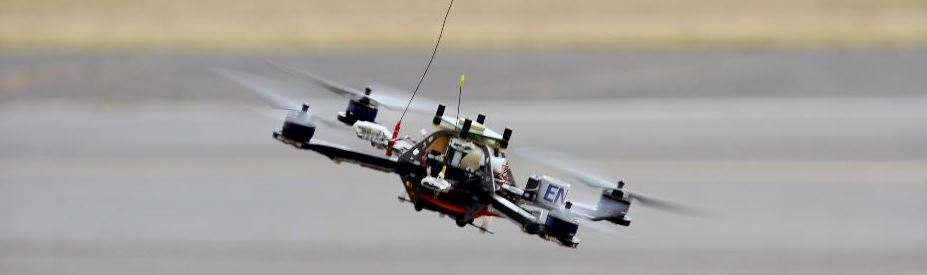
\includegraphics[width=\textwidth]{fig/mav}
	\caption{An example of a Quadrotor-\ac{MAV}-Platform that is used in this thesis.}
	\label{fig:mav}
\end{figure}

Especially in emergency scenarios the fast and safe flight of \acp{MAV} is crucial to deliver help quickly and save human lives. However, due to the complexity of such missions as well as the difficulty to control an \ac{MAV} in disaster scenarios, often multiple human operators are required in order to ensure safe operation \cite{Murphy2016}. With humans in the loop a constant connection between the \ac{MAV} and the operators is required which not only uses energy and requires infrastructure but also significantly increases the reaction time. Enabling \acp{MAV} to fly more autonomously could allow human operators to control more \acp{MAV} and thus to improve the support in emergency situations.

A major challenge on the way to the full autonomous flight of \acp{MAV} is the accurate estimation of the \ac{MAV}'s state within its environment. The system is highly dynamic so position and orientation can change rapidly. At the same time noise introduced by motor vibrations makes the position estimation with only on-board \acp{IMU} too inaccurate \cite{Mohamed2014}. \ac{LIDAR}-sensors can capture long and wide range 3D information but the sensors are typically heavy and require a significant amount of energy. \ac{IR} sensors can cover distance information but are often limited in their \ac{FoV} as well as in their range. External infrastructure like \ac{GPS} and optical tracking systems can provide accurate measurements but there is no guarantee that such systems are present in real world applications. Cameras on the other hand are cheap, lightweight and can measure long range distance information. This makes them a suitable choice as a sensor for on-board state estimation on light \acp{MAV} \cite{Elbanhawi2017}.

However, the signal delivered by the camera is high dimensional and can not directly be interpreted as position or orientation measurements. Computer Vision algorithms are required to interpret the image and extract relevant information. This can be done by designing an algorithm manually or learning the image processing from annotated examples. In particular Deep Learning based methods aim to combine whole Computer Vision pipelines into one mapping that transforms the raw input image into a task dependent output. Experiments have shown how Deep Learning based methods outperform traditional Machine Learning approaches and manually crafted algorithms \cite{Razavian}. This made them the predominant choice for almost any vision task.

The hereby used \acp{CNN} are designed in a hierarchical way, using multiple layers that are evaluated sequentially. An example architecture is displayed in \Cref{fig:cnn_example}. The network transforms an image of size 224x224 from its input (left) to a task dependent output (right). In this case a classification network predicting 1000 class probabilities is displayed. Each layer applies a non-linear transformation for which the parameters are learned during training. By stacking more layers on top of each other (deepening) and increasing the number of nodes $D$ per layer (widening), highly non-linear functions can be modelled. 

Experiments have shown the superior performance of particularly deep/wide models \cite{He, He2015, Szegedy2014, Zagoruyko2016}. However, this model flexibility assumed to be the reason for their superior performance also leads to immense requirements in computational resources. For example a state-of-the-art Computer Vision model \cite{He2015} contains 60.2 million parameters and one inference requires 11.3 billion floating point operations \cite{Tschannen2017}. 

\begin{figure}[bhtp]
	\centering
	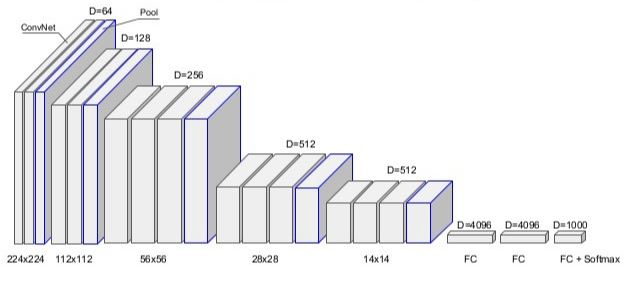
\includegraphics[width=0.8\textwidth]{fig/vgg_architecture}
	\caption{Example Architecture of a \ac{CNN}.}
	\label{fig:cnn_example}
\end{figure}

Robotic platforms like \acp{MAV} have limited resources in terms of processing power and battery life. Hence, the use of \acp{CNN} on such devices is still an open challenge. Research has addressed to reduce the number of computations in Deep Learning models on multiple levels\cite{YoungwanLee, Zagoruyko2016, Howard2017, Ghosh2017, Sandler2018, Zhang2017a}. However, the investigation of relatively shallow models with less than ten layers received only little attention by the research community.

This work investigates the deployment of a Deep Learning based Computer Vision pipeline on a \ac{MAV}. The method is applied in the challenging scenario of Autonomous Drone Racing at the \ac{IROS} 2018. Within the race court several metal gates are placed and need to be passed one after another. Detecting the gates allows to estimate the \ac{MAV}'s relative position and to calculate the flying trajectory. An overview of the race court and the racing gates at the \ac{IROS} 2016 Autonomous Drone Race can be seen in \Cref{fig:race_court}.

\begin{figure}[bhtp]
	\centering
	\begin{minipage}{0.45\linewidth}
	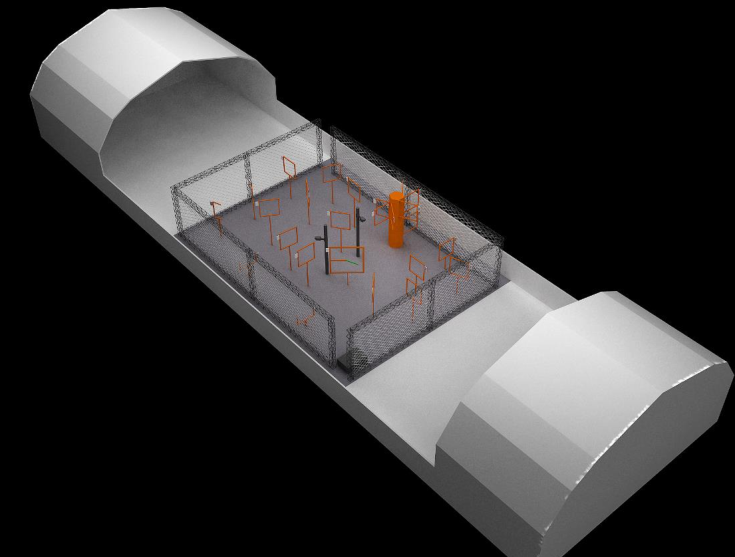
\includegraphics[width=\textwidth]{fig/race_court}
	\end{minipage}\hfill
\begin{minipage}{0.45\linewidth}
	\includegraphics[width=\textwidth]{fig/race_court_side}
\end{minipage}
\caption{Example Images of the \ac{IROS} 2016 Autonomous Drone Race}
\label{fig:race_court}
\end{figure}

The thesis builds on previous work by Ozo et. al \todoref{Reference to Current Method once it is published} which uses a manually crafted image processing method to detect the racing gates. Although fast to execute the method is very sensitive to illumination changes. Moreover, the algorithm fails when the objects are too far away or the frame is very thin. In order to develop a more robust method, this thesis investigates a learning based approach to the detection of racing gates.

Object Detection is one of the most intensively studied topics in Computer Vision. However, the objects investigated are usually solid and contain complex shapes. For example a pedestrian consist of body parts and a face. A box that surrounds the object mostly contains parts with distinctive shape an/or texture. A Computer Vision model can use these features for detection. The racing gates in contrast are of different nature. As can be seen in \Cref{fig:race_court} a box that surrounds the object would largely contain background. Hence, this part can not be used as a hint whether an object is present. Instead it can contain other objects even other gates that might distract a detector. Additionally, the object parts themselves are of very thin structure and can be hardly visible. Thus, a detector needs to make use of fine-grain structures, while ignoring the majority of the image. This introduces a particular vision task that even humans have a hard time at solving \footnote{The unconvinced reader can try to count the number of gates visible in the right image of \Cref{fig:race_court}} and that affects the training and design of a Computer Vision pipeline that aims to detect these kind of objects.

This thesis defines a class of objects as \textbf{\ac{EWFO}} studies methods for their detection. The definition is given as follows:

\paragraph{Definition - Empty Wireframe Objects}	
\begin{enumerate}
	\item \textbf{Empty.} The object parts are sparse. The bounding box around the object is largely occupied by background.
	\item \textbf{Wireframe} The object does not consist of complex but only basic geometric shapes like corners, lines and edges. The object parts can be spread over large parts of the image.

\end{enumerate}

The detection of \ac{EWFO} is studied in the examples of the \ac{IROS} drone race gates. These can be seen can be seen in \Cref{fig:gates}. The image shows the \textit{Closed Gate} as well as the \textit{Jungle Gate}. Thereby the orange part is considered to be the object of interest. To the best of the authors knowledge \ac{EWFO} have not been particularly addressed in Computer Vision. In \cite{Falanga} and \cite{Li2018a} the authors also detect racing gates, however the used objects contain more structure than the ones investigated in this thesis. \citeauthor{Jung2018} present a framework to detect similar objects in \cite{Jung} and \cite{Jung2018} but do not study the particular effects of the object shape. This work particularly addresses the implications of the object shape in using a Deep Learning based detection system for \ac{EWFO}.

\begin{figure}[bhtp]
	\centering
	\begin{minipage}{0.45\linewidth}
		\centering
		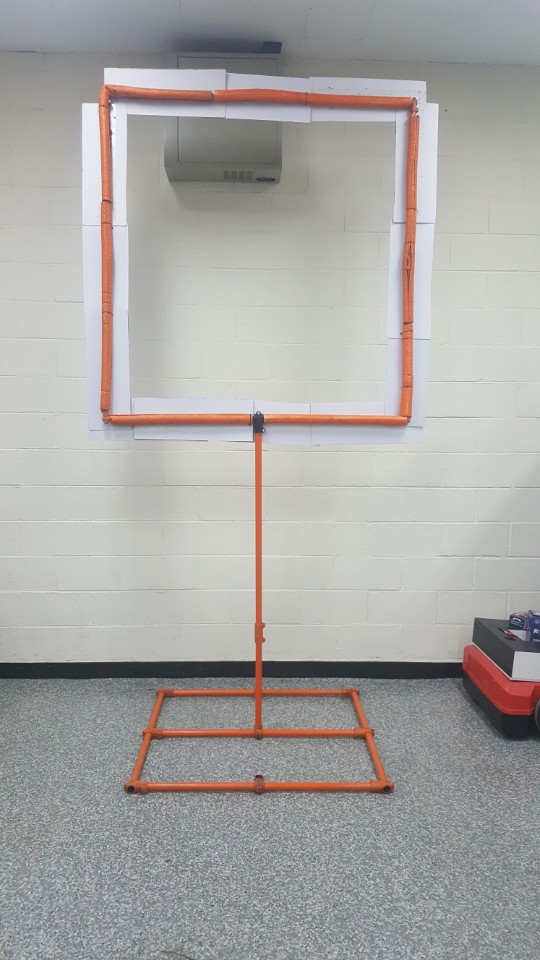
\includegraphics[height=5cm]{fig/closed_real}
	\end{minipage}\hfill
	\begin{minipage}{0.45\linewidth}
		\centering
		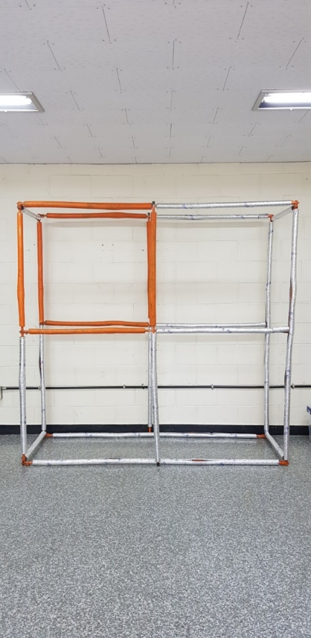
\includegraphics[height=5cm]{fig/jungle_real}
	\end{minipage}
	\caption{Example Images of the Empty Wire Frame Objects investigated in this thesis. }
	\label{fig:gates}
\end{figure}

A drawback of Deep Learning based vision systems is their need for vast amounts of annotated examples, which is not always available. Racing gates for example are not an object that appears often in everyday life and therefore not many example images exist. To this end no publicly available dataset can be used to train a Computer Vision system for \ac{EWFO}. Since a large part of the object consists of background, it is particularly crucial that the training set covers a large variety of backgrounds. Otherwise, it is likely that a model uses the background for prediction and only works in a particular domain (Overfitting). 

\begin{figure}[bhtp]
	\begin{minipage}{0.49\textwidth}
		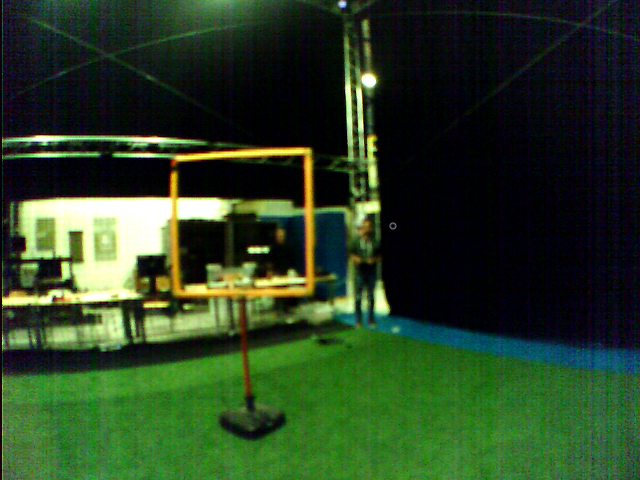
\includegraphics[width=\textwidth]{fig/real_cyberzoo2}
	\end{minipage}
	\begin{minipage}{0.49\textwidth}
		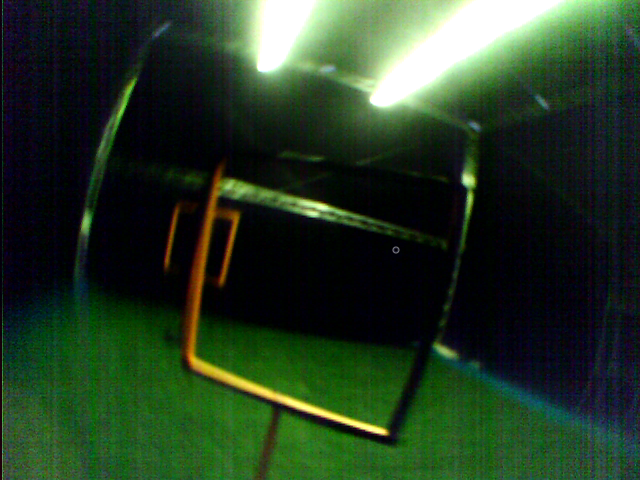
\includegraphics[width=\textwidth]{fig/real_cyberzoo1}
	\end{minipage}
	\label{fig:examples}
	\caption{Example of the \text{Cyberzoo} dataset. On the left an image while the \ac{MAV} is hovering, on the right an image during a turn manoevre.}
\end{figure}

In \Cref{fig:examples} example images of the target domain of this work are displayed. The images are taken during a test flight at a test environment. The left image shows an example when the \ac{MAV} is hovering and thus is in a very stable position. The object in this case is clearly visible as a single orange square. In contrast the right image shows a close up example during a turn manoeuvre. Here it can be seen how the used wide angle lens causes distortion and thus the lines appear as circular shape. Furthermore, large parts of the image including the horizontal bars of the object in the back appear blurred due to the circular velocity of the \ac{MAV}. In addition, the light conditions of the environment significantly influence the object appearance.

While it is possible to remove lens and sensor effects in post-processing, this can lead to information loss and requires on-board resources. Instead it is computationally more efficient to perform the detection on the raw image data. However, sensor effects have been shown to significantly influence the performance of neural networks \cite{Andreopoulos2012,Dodge2016a}. Furthermore, they can lead to varying object appearance on different \acp{MAV}. This further complicates the collection of annotated examples.
 
Another option is the artificial generation of data. By synthetically generating samples with corresponding labels, the theoretical amount of training data is infinite. Moreover, the generation allows to incorporate domain specific properties such as motion blur or image distortion. Hence, data generation is particularly useful for the detection of \acp{MAV} on \acp{EWFO} where a large variety of backgrounds is required while samples are difficult to obtain. Finally, as \ac{MAV} are brittle vehicles and mistakes in development can lead to damage on hardware, engineers and researchers often use simulators to evaluate their systems before transferring them to the real work. Thus the basic infrastructure required to generate data is often already available. 

Yet introduces the generation of data its own challenges. First and foremost because the generation process in itself is based on model assumptions. If these do not sufficiently capture the real world, a model trained in such an environment might be heavily biased and perform poorly in the real world. Secondly, because the generation of visual data is computationally intense. Despite advances in Computer Graphics can virtual environments not yet fully capture the real world. Hence, this work investigates the use of data generation in order to detect \acp{EWFO} on \acp{MAV}.

Without an accurate detection of the racing gate, the \ac{MAV} is not able to determine its current position and thus to calculate its flying trajectory. On the other hand, with an algorithm that requires less computational resources a lighter \ac{MAV} can be built. This allows faster and more aggressive trajectories as well as longer battery life. Moreover, the vision system is part of a greater state estimation and control system which also includes further sensor measurements. Depending on the remaining part of the system, faster and less accurate detections can be more useful than slow but accurate detections. Hence, the trade-off between accuracy and inference speed is of particular interest for this application and is addressed in this work.

\section{Research Question}

This section summarizes the research question addressed in this thesis. Furthermore it describes how the question is split in multiple subquestions that are addressed in the individual chapters.

	\textbf{How can \acp{CNN} detect \ac{EWFO} on \acp{MAV}, using synthetic training data?}


\begin{enumerate}
	\item[\textbf{RQ1}]How can data be generated to train a detection model for \ac{EWFO} detection on a \acp{MAV}?
	\item[\textbf{RQ2}]What kind of architecture is suitable to detect \acp{EWFO}?
	\item[\textbf{RQ3}]What are the trade-offs in detection performance and inference time when a detection model for \acp{EWFO} is deployed on a \ac{MAV}?
	\item[\textbf{RQ4}]Can the gained insights be used to build a lightweight and robust detection model for racing gates in the \ac{IROS} Autonomous Drone Race?
\end{enumerate}

\section{Results/Contributions}

\todo{Put some results at the end.}

\section{Outline}

\todo{Refactor contributions once done}
\begin{figure}[hbtp]
	\centering
	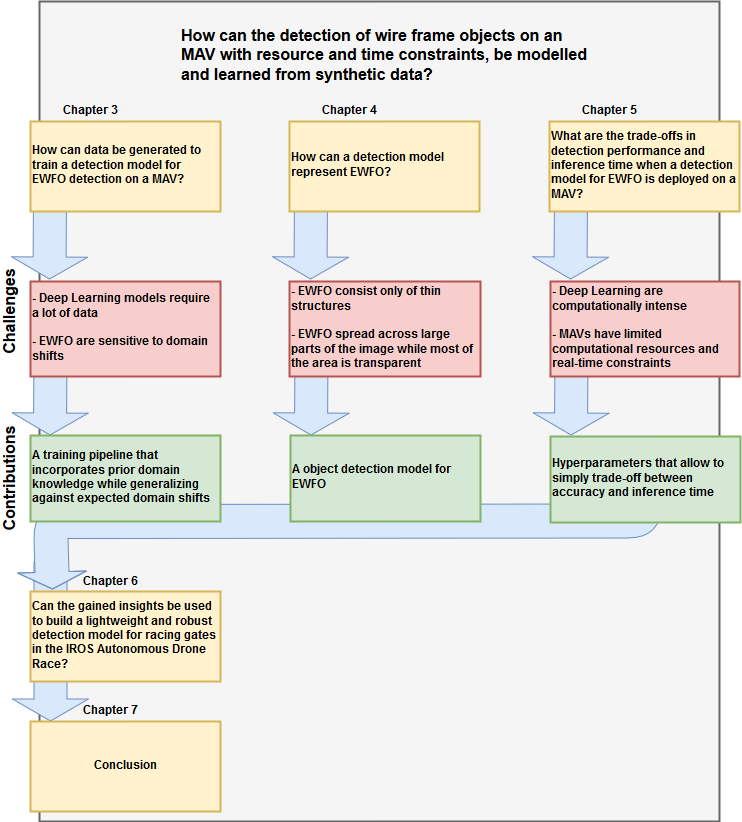
\includegraphics[width=\textwidth]{fig/Outline}
	\caption{Thesis Outline}
	\label{fig:outline}
\end{figure}


The thesis is structured as displayed in \Cref{fig:outline}. \Cref{sec:metrics} describes the metrics and systems used for evaluation. \Cref{sec:training}, \Cref{sec:object_detection}, \Cref{sec:tradeoff} and \Cref{sec:method} address the individual research questions. Each chapter contains an introduction to the topic, the methodology used in this thesis and experiments that have been carried out. \Cref{sec:training} describes methods to generate synthetic data for machine learning. It concludes with the datasets used for the remaining parts of this thesis.  \Cref{sec:object_detection} describes object detection and evaluates current methods in the application for \acp{EWFO}. \Cref{sec:tradeoff} illustrates and evaluates measures to reduce computations and optimize an object detection system for a particular hardware. It investigates the trade-off between detection performance and inference time. \Cref{sec:method} describes how the gained insights are used to develop a detector for racing gates at the \ac{IROS} 2018 Autonomous Drone Race. It also compares the current method to a traditional image processing method in terms of speed and detection performance. \Cref{sec:disc} discusses the overall results and formulates a conclusion.



